\documentclass{article}
\usepackage{amsmath}
\usepackage{url}
\usepackage{graphicx}
\usepackage{subcaption}
\title{Solving Symplectic Problem}
\author{Feng Zhao}

\begin{document}
\maketitle
I use Midpoint to solve the problem with the stepsize $h=0.1$.
One is explicit Midpoint and the other is implicit.
The evolution of the energy $\frac{p^2+q^2}{2}$ is shown in
Figure \ref{fig:e}. It can be seen that
the energy obtained explicit Midpoint at each time steps diverges gradually
while that of implicit Midpoint is preserved.
\begin{figure}[!ht]
    \centering
    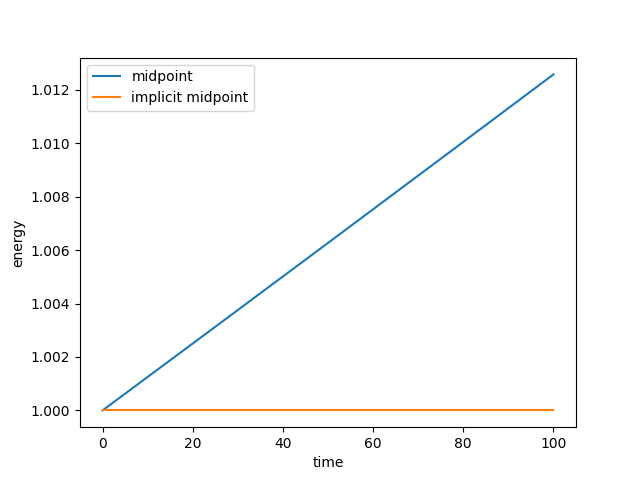
\includegraphics[width=5cm]{energy.png}
    \caption{Energy evolution for symplectic and non-symplectic methods}
    \label{fig:e}
\end{figure}
Though implicit midpoint can preserve the energy much better,
the global error is still accumulated as time passes by.
This error comes from the phase delay, which is shown more clearly
if when choose $T=1000$ (See Fig \ref{fig:o}).

\begin{figure}[!ht]
    \centering
    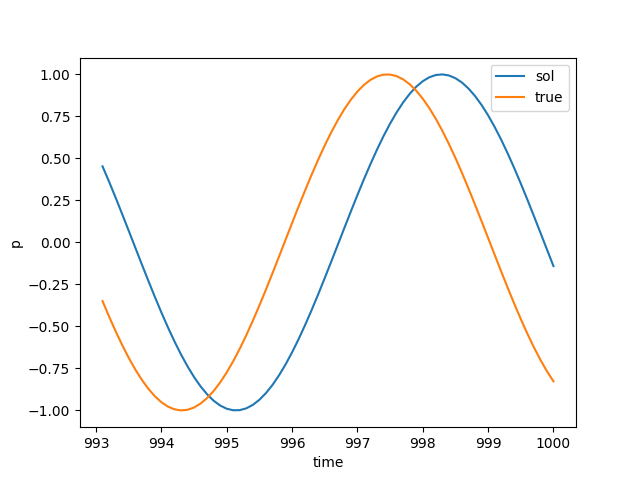
\includegraphics[width=5cm]{phase_delay.png}
    \caption{Origin of the global error for \texttt{ImplicitMidpoint}:
    the blue line is the true solution $p=-\sin(t)$ while
    the orange one is the numerical solution.}
    \label{fig:o}
\end{figure}


\end{document}



